% Manuscript draft generated from the experiment files in experiment/preseen/ (SPEC.md, LOG.md, config.yaml,
% committee/, questions/, people/, cards/, preseen_exp/, results/). Compiles with pdfLaTeX, XeLaTeX or LuaLaTeX.
\documentclass[11pt]{article}
\usepackage{iftex}
\ifPDFTeX
  \usepackage[T1]{fontenc}
  \usepackage[utf8]{inputenc}
  \usepackage{lmodern}
  \DeclareUnicodeCharacter{2010}{-}
  \DeclareUnicodeCharacter{2212}{-}
  \DeclareUnicodeCharacter{2264}{\ensuremath{\le}}
  \DeclareUnicodeCharacter{2265}{\ensuremath{\ge}}
  \DeclareUnicodeCharacter{00D7}{\ensuremath{\times}}
  \DeclareUnicodeCharacter{2192}{\ensuremath{\rightarrow}}
\else
  \usepackage{fontspec}
\fi
\usepackage[margin=1in]{geometry}
\usepackage{amsmath,amssymb}
\usepackage{booktabs,longtable,tabularx,array,multirow}
\usepackage{xcolor}
\usepackage{fvextra}
\usepackage{enumitem}
\usepackage{caption}
\usepackage{tikz}
\usetikzlibrary{positioning,arrows.meta}
\usepackage[hidelinks]{hyperref}
\usepackage{microtype}
\usepackage{graphicx}
\setlength{\emergencystretch}{3em}
\setlength{\LTcapwidth}{\textwidth}
\fvset{breaklines=true,breakanywhere=true,fontsize=\footnotesize,frame=single,framesep=2mm}
\newcolumntype{L}{>{\raggedright\arraybackslash}X}
\newcommand{\code}[1]{\texttt{\detokenize{#1}}}
\title{Do bibliometric profiles change an AI forecaster's view of the Nobel Prize?\\[4pt]
\large A controlled context experiment on the 2026 Nobel Prizes in Physiology or Medicine, Physics and Chemistry\\[2pt]
\normalsize Design, implementation and status report}
\author{Dawoon Jeong}
\date{Draft of 1 October 2026, status as of 18:15 CDT}
\begin{document}
\maketitle
\begin{abstract}
\noindent
We test whether structured bibliometric profiles of the scientists named in a forecasting question change the
probabilities that an AI forecasting system (Preseen) assigns to the possible outcomes of the 2026 Nobel Prizes in
Physiology or Medicine, Physics and Chemistry. For each field, a virtual Nobel committee---personas that mirror the
specialties of the actual 2026 Nobel Committee, each run on three large language models from different providers
(Anthropic \code{claude-opus-5-5}, OpenAI \code{gpt-5.5-2026-04-23}, Google \code{gemini-3.1-pro-preview})---produced
ranked nominations, which were aggregated by a model-balanced Borda count into twelve candidate discoveries plus
``Other''. The same multiple-choice question was created twice on Preseen: a control question without context and a
treatment question carrying one context note per named person (98 profile cards in total), built from an author-profile pipeline over the OpenAlex 2026-01 snapshot, PatentsView
2025-12-31 and Reliance on Science. Each card compares the person with the field's 2000--2025 laureates measured at the
time of their prize. Repeated, interleaved runs of both questions estimate the treatment effect against the run-to-run
spread of the control. The committee stage (66 ballots,
all valid) cost about \$7.12; all profiles and cards are complete; at the time of writing the
Preseen runs are in progress. This document records the protocol, every decision taken during implementation, the
deviations from the protocol and their reasons, and the results available so far.
\end{abstract}

\tableofcontents
\newpage
\section{Introduction}

AI forecasting systems increasingly answer questions about future events by searching, reading and synthesising
evidence. A natural question is how much such a system's forecast depends on what it is given to read. Scientific
prizes are a good test case: the outcome is a discrete choice among a small set of discoveries, the decision process is
well documented, the outcome is announced on a known date, and rich quantitative descriptions of the candidates'
work exist. We ask a narrow, testable question:

\begin{quote}
\emph{When a forecasting system is given neutral, descriptive bibliometric profiles of the people named in each option,
do its probabilities for the 2026 Nobel Prizes move by more than they move between repeated runs without the
profiles?}
\end{quote}

The experiment is built so that the only difference between the arms is the context attached to the question. The
candidate discoveries themselves are generated independently of the profiles and of the forecasting system by a
virtual committee of language-model personas. The profiles are produced by an existing pipeline that profiles any
scientist with an OpenAlex author record, and are reduced to fixed-template cards of 300--500 words that state
measures and comparisons but no prediction.

\paragraph{The prize process in brief.} Alfred Nobel's will rewards ``the most important discovery'' in physiology or
medicine, ``the most important discovery or invention'' in physics and ``the most important chemical discovery or
improvement''. The Statutes of the Nobel Foundation limit a prize to at most three people, allow it to be divided
between two works, and, since 1974, exclude posthumous awards (unless death occurs after the announcement). The unit
of the prize is therefore the discovery, summarised in the official prize motivation, and the forecasting question is
framed at that level. The 2026 announcements are scheduled for 5 October (Physiology or Medicine), 6 October (Physics)
and 7 October (Chemistry).

\paragraph{Contributions of this document.} (i) A complete protocol (Sections~\ref{sec:design}--\ref{sec:analysis});
(ii) the full record of implementation decisions, including manual merge and identity decisions with their reasons
(Sections~\ref{sec:committee}--\ref{sec:cards}, Appendices); (iii) incidents and deviations from the protocol
(Section~\ref{sec:deviations}); (iv) results available at the time of writing (Section~\ref{sec:results}).
\section{Design}\label{sec:design}

\begin{figure}[ht]
\centering
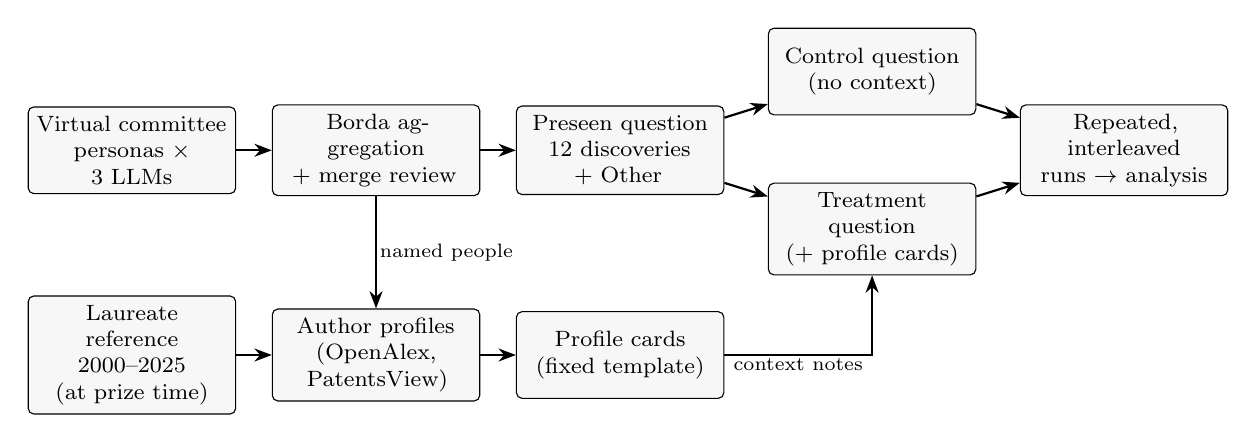
\begin{tikzpicture}[every node/.style={font=\footnotesize, align=center},
  box/.style={draw, rounded corners=2pt, minimum height=11mm, text width=24mm, fill=black!3},
  arr/.style={-{Stealth[length=2.2mm]}, thick}, lab/.style={font=\scriptsize, fill=white, inner sep=1pt}]
\node[box] (c) at (0,0) {Virtual committee\\personas $\times$ 3 LLMs};
\node[box] (a) at (3.1,0) {Borda aggregation\\+ merge review};
\node[box] (q) at (6.2,0) {Preseen question\\12 discoveries\\+ Other};
\node[box] (ctl) at (9.4,1.0) {Control question\\(no context)};
\node[box] (trt) at (9.4,-1.0) {Treatment question\\(+ profile cards)};
\node[box] (runs) at (12.6,0) {Repeated, interleaved\\runs $\rightarrow$ analysis};
\node[box] (p) at (3.1,-2.6) {Author profiles\\(OpenAlex,\\PatentsView)};
\node[box] (r) at (0,-2.6) {Laureate reference\\2000--2025\\(at prize time)};
\node[box] (cards) at (6.2,-2.6) {Profile cards\\(fixed template)};
\draw[arr] (c) -- (a); \draw[arr] (a) -- (q);
\draw[arr] (q) -- (ctl); \draw[arr] (q) -- (trt);
\draw[arr] (ctl) -- (runs); \draw[arr] (trt) -- (runs);
\draw[arr] (a) -- node[lab, right]{named people} (p);
\draw[arr] (r) -- (p); \draw[arr] (p) -- (cards);
\draw[arr] (cards) -| node[lab, pos=0.25, below]{context notes} (trt);
\end{tikzpicture}
\caption{Pipeline of the experiment, run separately for each field. The committee never sees the profiles or any
Preseen output; the question text never mentions the committee, the models, the profiles or the experiment.}
\label{fig:pipeline}
\end{figure}

For each field $F\in\{\text{Physiology or Medicine},\ \text{Physics},\ \text{Chemistry}\}$:

\begin{enumerate}[leftmargin=*]
\item \textbf{Virtual committee.} Personas mirror the specialties of the actual 2026 Nobel Committee of the field
(Medicine 6, Physics 8, Chemistry 8). Every persona is run on three language models from different providers (a crossed
persona $\times$ model design), producing up to five ranked nominations. A model-balanced Borda count aggregates the
ballots into twelve candidate discoveries plus ``Other''.
\item \textbf{Preseen multiple-choice question}, created twice with identical definitions: \emph{control} (no context)
and \emph{treat} (one context note per named person plus a definitions note, all with \code{treatment=consider}). A
placebo arm (\emph{shuffle}: the same cards with the numeric block deranged across persons) is implemented as an option
and switched off (\code{placebo: false}).
\item \textbf{Repeated, interleaved runs.} One control run is made before any context is added (a ``first look'');
after the context is ready, three further runs per arm are submitted in a randomised, interleaved order. The treatment
effect per option is compared with the run-to-run spread of the control arm.
\end{enumerate}

\paragraph{Why one question per arm.} Preseen context notes are attached to a question and apply to every later run
of it; there is no per-run override. Separate, identically defined questions are therefore the only way to hold the
question fixed while varying the context. The client checks after creation that the stored definitions of the arms are
identical.

\paragraph{Why a crossed committee.} Running every persona on every model gives each model equal weight, separates
persona effects from model effects, and makes agreement between models a diagnostic. Models trained on overlapping
data remain correlated; the crossed design reduces, but does not remove, that correlation.

\paragraph{Independence.} The committee never sees profiles, cards or Preseen output and uses no tools, web search
or grounding. The question's title, description and resolution criteria are neutral, identical across arms, and checked
automatically against a list of forbidden words (\code{committee}, \code{model}, \code{profile}, \code{experiment},
\code{Preseen}, \ldots).

\paragraph{Deadlines.} No forecast may run after its prize is announced. All runs of a field must finish by 23:00 CDT
on the evening before its announcement (Table~\ref{tab:deadlines}).

\begin{table}[ht]\centering\small
\caption{Fields, tags and deadlines (times CDT).}\label{tab:deadlines}
\resizebox{\textwidth}{!}{\begin{tabular}{lllll}\toprule
Field & Announcement (earliest) & Runs finished by & Tag & Committee size\\\midrule
Physiology or Medicine & Mon 05 Oct, 04:30 & Sun 04 Oct, 23:00 & \code{nobel26-med} & 6\\
Physics & Tue 06 Oct, 04:45 & Mon 05 Oct, 23:00 & \code{nobel26-phys} & 8\\
Chemistry & Wed 07 Oct, 04:45 & Tue 06 Oct, 23:00 & \code{nobel26-chem} & 8\\
\bottomrule\end{tabular}}\end{table}
\section{The virtual Nobel committee}\label{sec:committee}

\subsection{Personas}

Each persona is ``a senior member of the Nobel Committee for $\langle$field$\rangle$ whose own expertise is
$\langle$specialty$\rangle$''. Only the specialties of the real 2026 committee members are used---no names, no
impersonation and no opinions attributed to real people. Because real committees cover gaps with expert advisers,
each persona uses its specialty as a lens but nominates across the whole field (Table~\ref{tab:personas}).

\begin{table}[ht]\centering\small
\caption{Persona specialties (from the 2026 committee rosters).}\label{tab:personas}
\begin{tabularx}{\textwidth}{lL}\toprule
Field & Specialties\\\midrule
Physiology or Medicine (6) & neurology; molecular systems biology; neuroscience; molecular genetics; experimental rheumatology (immunology, autoimmunity); molecular developmental biology\\
Physics (8) & astroparticle physics; theoretical magnetism; applied and theoretical quantum physics; atomic physics; general physics; theoretical physics; complex systems; experimental physics, microscopy and microanalysis\\
Chemistry (8) & nanophysics; medical biochemistry; organic chemistry; physical chemistry; inorganic and structural chemistry; molecular physics; biochemistry; theoretical chemistry\\
\bottomrule\end{tabularx}\end{table}

\subsection{Models and calls}

One model per provider was chosen at the first checkpoint and fixed for all three fields:
Anthropic \code{claude-opus-5-5}, OpenAI \code{gpt-5.5-2026-04-23} (a dated snapshot) and Google
\code{gemini-3.1-pro-preview}. All calls use plain HTTPS (Python \code{requests}; no SDKs):
Anthropic \code{/v1/messages} with \code{output_config.format} (JSON schema); OpenAI \code{/v1/responses} with a strict
\code{json_schema} text format and \code{store=false}; Gemini \code{generateContent} with \code{responseJsonSchema}.
The same system and user text go to every provider; only the envelope differs. No tools, no web search, no grounding,
no sampling parameters and no reasoning or effort settings are sent, so each provider runs with its defaults (reported
defaults: OpenAI temperature 1.0, top\_p 0.98, reasoning effort medium; Anthropic: adaptive thinking, documented
default effort medium; Gemini: default thinking). No server-side model fallback is enabled, since it would replace the
model inside a cell. The output cap is 32{,}000 tokens (billed by use). Every response's reported model string is
recorded; all equal the requested ids.

\paragraph{Validation and retries.} Each ballot is parsed and validated locally: structure and types are hard
requirements; count limits (at most 5 nominations, 1--3 people, at most 3 key papers, at most two sentences of
rationale) are recorded as warnings. A ballot that is not valid JSON for the schema is asked once more; a cell that
still fails is recorded as missing and never re-asked silently. Transient HTTP errors (408, 429, 5xx) are retried with
back-off; a 429 whose message reports a zero quota is not retried.

\subsection{Prompt}

The prompt (Appendix~\ref{app:prompt} reproduces it verbatim for one persona) contains: the persona; the date context
(``late September 2026; the 2026 prize has not been announced''); the rules that matter (the will's wording for the
field, at most three living laureates, a possible division between two discoveries); the field's prizes 2000--2025 with
their official motivations and laureates, taken from PrizeAtlas (one line per prize share; Medicine 29 lines, Physics 35,
Chemistry 31); and the task: up to five ranked nominations, each with a one-line discovery in the style of a Nobel
motivation, one to three living people with affiliations, up to three key papers if known, and a rationale of at most
two sentences, returned as one JSON object.

\subsection{Test ballots and cost}

One test ballot per model (Medicine, neurology persona) checked the prompt, the parsing and the cost before the full
run. The Gemini key first returned HTTP 429 (free tier, zero quota for the model); after billing was enabled the call
succeeded. The full committee (all persona $\times$ model cells of the three fields) ran on 1 October 2026,
14:17--14:36 CDT, with two concurrent calls per provider. All 66 cells returned a valid ballot on the first attempt; two ballots carried a warning (a three-sentence rationale).

\begin{table}[ht]\centering\small
\caption{Committee token use and cost (all three fields; list prices per million tokens in parentheses).}\label{tab:cost}
\begin{tabular}{lrrr}\toprule
Model & Input tokens & Output tokens (incl.\ reasoning) & Cost (USD)\\\midrule
\code{claude-opus-5-5} (\$4 / \$20) & 60,176 & 72,791 & 1.70\\
\code{gpt-5.5-2026-04-23} (\$5 / \$30) & 33,152 & 134,585 & 4.20\\
\code{gemini-3.1-pro-preview} (\$2 / \$12) & 32,210 & 96,154 & 1.22\\
\midrule Total & 125,538 & 303,530 & 7.12\\
\bottomrule\end{tabular}\end{table}

\subsection{Aggregation}

\paragraph{Model-balanced Borda count.} A nomination at rank $r\in\{1,\dots,5\}$ earns $6-r$ points. Let $B_m$ be the
number of valid ballots of model $m$ in the field and $P_{m,j}$ the points that model $m$'s ballots give to option $j$.
The option score is
\begin{equation}
S_j=\sum_{m}\frac{P_{m,j}}{B_m},
\end{equation}
so every model contributes the same total (at most 15 points per ballot on average) regardless of missing cells.
Ties are broken by the number of models nominating the option, then by the number of nominations.

\paragraph{Merging nominations into options.} Nominations that describe the same discovery are merged.
\emph{Automatically}, nominations that share a person are linked, and the connected components form options. A person
is identified by first initial and surname (accents and punctuation folded); when one such key carries two different
middle initials (e.g.\ Charles H.\ Bennett, quantum information, and Charles L.\ Bennett, cosmic microwave background),
the key is split by middle initial and a name without middle initial is left unlinked. \emph{Manually}, a per-field file
(\code{committee/<field>/merges.yaml}) records, each with a written reason: \emph{splits} (nominations that leave their
automatic option), \emph{merges}, \emph{aliases} (spelling variants of a name), \emph{wording} (the option takes the
discovery wording of a named member nomination), \emph{people} (the shown people chosen by hand, used for ties) and
\emph{deceased} people (Section~\ref{sec:living}). Three rules guided the manual decisions: (1) an umbrella nomination
that spans two distinct discoveries and chains them together becomes an option of its own; (2) discoveries linked only
through one shared person are split; (3) when the automatic wording comes from an outlier member, the majority wording
is used. Every merge, automatic or manual, is listed with its reason in \code{review.md}; nominations whose wording
overlaps little with the rest of their option are marked for checking.

\paragraph{Option text.} The option text is the discovery (in the style of a prize motivation) followed by the three
people with the most normalised points within the option, e.g.\ ``for the discovery of glucagon-like peptide-1 and its
development into therapies for diabetes and obesity --- Svetlana Mojsov, Jens Juul Holst, Lotte Bjerre Knudsen''.

\subsection{Diagnostics}

For every field \code{review.md} reports per-model top-12 lists and their pairwise Jaccard overlap, the number of
cross-model-consensus options (nominated by all three models) and single-model options, leave-one-out stability (the
number of top-12 options that change when one persona or one model is dropped), and flags: possibly already awarded
(word overlap with a 2000--2025 motivation), Nobel laureates and deaths among the named people (PrizeAtlas), more than
three people, and a person in two options (Table~\ref{tab:diag}).

\begin{table}[ht]\centering\small
\caption{Committee diagnostics per field (A = Anthropic, O = OpenAI, G = Gemini).}\label{tab:diag}
\resizebox{\textwidth}{!}{\begin{tabular}{lrrrrrrl}\toprule
Field & Ballots & Nominations & Options & Jaccard A--O / A--G / O--G & Consensus & Single & Max LOO change\\\midrule
Physiology or Medicine & 18/18 & 90 & 22 & 0.33 / 0.28 / 0.44 & 4 & 1 & 3 of 12\\
Physics & 24/24 & 120 & 21 & 0.50 / 0.71 / 0.41 & 8 & 0 & 1 of 12\\
Chemistry & 24/24 & 120 & 28 & 0.41 / 0.33 / 0.41 & 6 & 0 & 3 of 12\\
\bottomrule\end{tabular}}\end{table}
\subsection{Manual merge decisions}

Table~\ref{tab:manual} summarises the manual decisions; Appendix~\ref{app:merges} lists them with their full reasons.
The most consequential were: Medicine---BRCA (King) and p53 (Lane, Levine, Vogelstein) had been chained through one
umbrella nomination naming both Vogelstein and King; Physics---quantum information (Bennett, Brassard, Shor), quantum
error correction (Shor, Steane, Kitaev), quantum spin liquids (Kitaev, Lee) and CMB cosmology (Charles L.\ Bennett) had
been chained through shared surnames; Chemistry---phosphoramidite DNA synthesis (Caruthers) and sequencing-by-synthesis
(Balasubramanian, Klenerman) had been chained through an umbrella nomination, and Buchwald--Hartwig coupling had been
linked to C--H functionalization only through Hartwig.

\begin{table}[ht]\centering\small
\caption{Number of manual decisions per field (\code{merges.yaml}).}\label{tab:manual}
\begin{tabular}{lrrrrrr}\toprule
Field & Splits & Merges & Aliases & Wording & People (ties) & Deceased\\\midrule
Physiology or Medicine & 2 & 0 & 0 & 0 & 1 & 2\\
Physics & 2 & 0 & 2 & 1 & 0 & 1\\
Chemistry & 4 & 0 & 2 & 2 & 2 & 0\\
\bottomrule\end{tabular}\end{table}
\subsection{Living check}\label{sec:living}

Because the prize is not awarded posthumously and the committee models' training data precede recent deaths, every
person shown in the three top-12 lists (95 people) was screened against Wikidata (date of death, P570; free read-only
API, paced to respect its rate limit), and every death, missing match, wrong match, replacement and everyone born in or
before 1940 was checked on the web. Three shown people had died and were replaced in the option text by the next living
person by weight (Table~\ref{tab:deceased}); the option itself is unchanged because the discovery can still be awarded
to living contributors. One Wikidata ``death'' was a namesake (a Jonathan Cohen who died in 2003); the PCSK9 geneticist
Jonathan C.\ Cohen is living. In all, eleven people (no Wikidata match, a wrong match, a replacement, or born $\le$ 1940)
were checked on the web, with no death notice found for any of them. A ``no death notice found'' is not proof of life; deaths after 1 October 2026 are not
covered.

\begin{table}[ht]\centering\small
\caption{Shown people found to be deceased and their replacements.}\label{tab:deceased}
\begin{tabularx}{\textwidth}{llllL}\toprule
Field & Option & Person & Died & Shown instead\\\midrule
Physiology or Medicine & GLP-1 & Joel F.\ Habener & 2025-12-28 & Lotte Bjerre Knudsen\\
Physiology or Medicine & CAR-T cell therapy & Zelig Eshhar & 2025-07-03 & Steven A.\ Rosenberg\\
Physics & aberration-corrected electron optics & Harald Rose & 2026-07-27 & Ondrej L.\ Krivanek\\
\bottomrule\end{tabularx}\end{table}

\subsection{Candidate lists}

Tables~\ref{tab:cand-medicine}--\ref{tab:cand-chemistry} give the final candidate lists (score $S_j$; $M$ = number
of models nominating; $P$ = number of personas nominating; \checkmark = nominated by all three models).
\begin{table}[ht]\centering\footnotesize
\caption{Candidate list, Physiology or Medicine (18 ballots; plus ``Other'').}\label{tab:cand-medicine}
\begin{tabularx}{\textwidth}{rLp{4.6cm}rrrc}\toprule
\# & Discovery & People shown & $S_j$ & $M$ & $P$ & \\\midrule
1 & Discovery of glucagon-like peptide-1 and its development into therapies for diabetes and obesity & Svetlana Mojsov, Jens Juul Holst, Lotte Bjerre Knudsen & 11.50 & 3 & 6 & \checkmark\\
2 & Development of optogenetics, a method to control the activity of genetically defined neurons with light & Karl Deisseroth, Peter Hegemann, Gero Miesenböck & 9.50 & 3 & 6 & \checkmark\\
3 & Development of chimeric antigen receptor T-cell therapy & Carl H. June, Michel Sadelain, Steven A. Rosenberg & 5.17 & 3 & 6 & \checkmark\\
4 & Discovery of the unfolded protein response & Kazutoshi Mori, Peter Walter & 2.67 & 2 & 6 & \\
5 & Discovery of PCSK9 and its role in regulating LDL cholesterol metabolism & Helen H. Hobbs, Nabil G. Seidah, Jonathan C. Cohen & 1.67 & 2 & 4 & \\
6 & Development of high-throughput next-generation DNA sequencing methods & David Klenerman, Shankar Balasubramanian & 1.67 & 1 & 2 & \\
7 & Discovery of orexin and its role in the regulation of sleep and wakefulness & Emmanuel Mignot, Masashi Yanagisawa, Luis de Lecea & 1.67 & 2 & 3 & \\
8 & Discoveries concerning the Wnt signaling pathway and its application in cultivating organoids & Hans Clevers, Roel Nusse & 1.50 & 2 & 1 & \\
9 & Discovery of leptin and the hormonal regulation of body weight & Jeffrey M. Friedman, Stephen O'Rahilly & 1.50 & 2 & 4 & \\
10 & Discovery of tumour necrosis factor as a therapeutic target in chronic inflammatory autoimmune disease & Marc Feldmann, Ravinder N. Maini & 1.33 & 3 & 1 & \checkmark\\
11 & Discovery of chaperone-mediated protein folding in cells & Arthur L. Horwich, Franz-Ulrich Hartl & 1.00 & 2 & 2 & \\
12 & Discovery of inherited susceptibility genes for breast and ovarian cancer & Mary-Claire King, Mark H. Skolnick, Michael R. Stratton & 0.83 & 2 & 2 & \\
\bottomrule\end{tabularx}\end{table}

\begin{table}[ht]\centering\footnotesize
\caption{Candidate list, Physics (24 ballots; plus ``Other'').}\label{tab:cand-physics}
\begin{tabularx}{\textwidth}{rLp{4.6cm}rrrc}\toprule
\# & Discovery & People shown & $S_j$ & $M$ & $P$ & \\\midrule
1 & Theoretical prediction and experimental discovery of topological insulators and the quantum spin Hall effect & Charles L. Kane, Eugene J. Mele, Laurens W. Molenkamp & 8.75 & 3 & 8 & \checkmark\\
2 & Invention and development of optical lattice clocks, enabling time and frequency measurements at unprecedented precision & Hidetoshi Katori, Jun Ye & 7.00 & 3 & 8 & \checkmark\\
3 & Theoretical prediction and experimental realization of negative index metamaterials & John B. Pendry, David R. Smith, Eli Yablonovitch & 5.12 & 3 & 8 & \checkmark\\
4 & Discovery of topological and geometric phases in quantum systems & Michael V. Berry, Yakir Aharonov & 4.12 & 3 & 6 & \checkmark\\
5 & Theoretical prediction and experimental discovery of correlated insulator behavior and superconductivity in magic-angle twisted bilayer graphene & Allan H. MacDonald, Pablo Jarillo-Herrero, Rafi Bistritzer & 3.00 & 3 & 8 & \checkmark\\
6 & Foundational discoveries in quantum information science, including quantum cryptography and quantum algorithms & Charles H. Bennett, Gilles Brassard, Peter W. Shor & 2.50 & 2 & 4 & \\
7 & Pioneering contributions to neutrino astronomy, in particular the discovery of high-energy cosmic neutrinos & Francis Halzen, Albrecht Karle, Naoko Kurahashi Neilson & 2.12 & 3 & 2 & \checkmark\\
8 & Observation of the shadow of a black hole by event-horizon-scale radio interferometry & Heino Falcke, Sheperd S. Doeleman, Katherine L. Bouman & 1.88 & 2 & 6 & \\
9 & Theoretical proposals and experimental realizations of quantum simulators using ultracold atoms in optical lattices & Immanuel Bloch, J. Ignacio Cirac, Peter Zoller & 1.88 & 2 & 4 & \\
10 & Invention of the quantum cascade laser & Alfred Y. Cho, Federico Capasso, Jérôme Faist & 1.75 & 2 & 5 & \\
11 & Invention of aberration-corrected electron optics, enabling electron microscopy with sub-ångström resolution & Maximilian Haider, Knut Urban, Ondrej L. Krivanek & 1.50 & 3 & 1 & \checkmark\\
12 & Theoretical formulation of cosmic inflation and the prediction of the quantum origin of cosmological structure & Alan H. Guth, Andrei Linde, Viatcheslav Mukhanov & 1.25 & 3 & 3 & \checkmark\\
\bottomrule\end{tabularx}\end{table}

\begin{table}[ht]\centering\footnotesize
\caption{Candidate list, Chemistry (24 ballots; plus ``Other'').}\label{tab:cand-chemistry}
\begin{tabularx}{\textwidth}{rLp{4.6cm}rrrc}\toprule
\# & Discovery & People shown & $S_j$ & $M$ & $P$ & \\\midrule
1 & Development of controlled radical polymerization & Krzysztof Matyjaszewski, Mitsuo Sawamoto, Ezio Rizzardo & 8.62 & 3 & 8 & \checkmark\\
2 & Development of massively parallel sequencing-by-synthesis of DNA & David Klenerman, Shankar Balasubramanian, Pascal Mayer & 8.62 & 3 & 8 & \checkmark\\
3 & Discovery and development of solid-state perovskite solar cells & Henry J. Snaith, Nam-Gyu Park, Tsutomu Miyasaka & 4.25 & 3 & 8 & \checkmark\\
4 & Development of phosphoramidite chemistry for automated DNA synthesis & Marvin H. Caruthers, Serge L. Beaucage, Mark D. Matteucci & 3.25 & 3 & 4 & \checkmark\\
5 & Development of transition-metal-catalyzed C-H functionalization reactions & John F. Hartwig, Jin-Quan Yu, Robert G. Bergman & 2.50 & 2 & 5 & \\
6 & Development of polymeric and lipid nanoparticle systems for the delivery of drugs and nucleic acids & Pieter R. Cullis, Robert S. Langer, Kazunori Kataoka & 2.38 & 2 & 8 & \\
7 & Discovery of targeted protein degradation by small molecules that redirect ubiquitin ligases & Craig M. Crews, Raymond J. Deshaies, Stuart L. Schreiber & 1.88 & 3 & 5 & \checkmark\\
8 & Discovery of molecular chaperones that assist protein folding in the cell & Arthur L. Horwich, F. Ulrich Hartl & 1.75 & 2 & 2 & \\
9 & Development of nanopore methods for single-molecule analysis and sequencing of nucleic acids & David W. Deamer, Hagan Bayley, Daniel Branton & 1.62 & 2 & 3 & \\
10 & Development of ab initio molecular dynamics & Michele Parrinello, Roberto Car & 1.50 & 3 & 3 & \checkmark\\
11 & Development of efficient organic light-emitting diodes & Ching W. Tang, Steven A. Van Slyke, Mark E. Thompson & 1.12 & 2 & 4 & \\
12 & Development of DNA origami and programmable self-assembly of DNA nanostructures & Paul W. K. Rothemund, William M. Shih, Hao Yan & 1.12 & 2 & 2 & \\
\bottomrule\end{tabularx}\end{table}

\section{The forecasting question}\label{sec:question}

The question is a private multiple-choice question with mutually exclusive and comprehensive options: the twelve
option texts of the candidate list plus ``Other''. Title, description and resolution criteria come from templates
shared by the three fields; for Physiology or Medicine they read:

\begin{description}[leftmargin=1.5em, style=nextline]
\item[Title] Which discovery will the 2026 Nobel Prize in Physiology or Medicine be awarded for?
\item[Description] The 2026 Nobel Prize in Physiology or Medicine is scheduled to be announced on Monday 5 October 2026. Each option names a discovery and the people most closely associated with it.
\item[Resolution criteria] Resolves to the option whose discovery matches the discovery named in the official motivation of the 2026 Nobel Prize in Physiology or Medicine, as published at nobelprize.org. Options are matched by discovery; the people named in an option need not match the laureates exactly. If the prize is divided between two discoveries, only the discovery with the larger share counts; if the shares are equal, the discovery named first in the announcement counts. If no option matches that discovery, the question resolves to Other.
\end{description}

Options are matched by discovery, not by people, because the committee cannot know which three people the Nobel
Assembly or Academy will choose. Option texts are kept exactly as approved after the committee review (in the style of
a prize motivation, starting with ``for the \ldots''). Preseen stores multiple-choice options as plain strings; the
longest option (Physics) has 213 characters and was accepted. The full Medicine question is in
Appendix~\ref{app:question}.
\section{Author profiles}\label{sec:profiles}

\subsection{The profile pipeline}

The repository's name pipeline (\code{pipeline/profile_person.py}) resolves a name to OpenAlex author ids (the 2026-01
snapshot's authors table, optionally the live OpenAlex author search, PrizeAtlas ids and ORCIDs for laureates), adds
same-name fragments of the chosen author, and runs a notebook on a Slurm compute node that writes a dashboard, an
agent-readable record and per-author tables: every work and patent scored against its cohort (citations,
disruption, Foundation / Extension / Generalization, citations from books), patent-to-paper citations, and
co-authorship, co-invention, institution and assignee networks. The window is works published, and patents granted,
up to 2021.

\subsection{Identity resolution}

The people file of each field (\code{people/<field>.txt}) lists every person shown in the options with the affiliation
the committee gave (98 rows, 94 distinct people; Klenerman, Balasubramanian, Horwich and Hartl appear in two fields).
A dry run resolves each name without profiling it. Because the pipeline's command-line dry run scans the 6~GB
snapshot authors table once per person (about 1.5 minutes each), a faster runner calls the pipeline's own, unchanged
resolution function on a one-scan subset of the authors table (all rows whose names contain one of the surnames, the
same substring test the resolver applies). For the 11 Medicine people that both runs had finished, ids, choice rule and
unresolved cases were identical.

Every unresolved or doubtful pick was reviewed with the candidate tables, single-author OpenAlex lookups (topics,
institutions) and the public ORCID API. Sixteen people were decided by hand (Appendix~\ref{app:identity}): seven
namesake cases without an automatic pick, eight automatic picks of small fragments, and one failed name search
(the apostrophe in O'Rahilly). Two cases merit mention. For Emmanuel Mignot the larger OpenAlex profile carries the
ORCID of Juliette Mignot, a climate scientist, and mixes two people; the Stanford profile with his own ORCID was used,
accepting an undercount. For Ching W.\ Tang and Steven A.\ Van Slyke, OpenAlex splits each person across several ids;
the ids with OLED topics were combined. The identity table (\code{people/<field>_identity.csv}) records, per person,
the options, chosen ids and choice rule, ORCID, institution, works and citations, prior Nobel prizes (none) and the
expected source of the inventor ids (the pqrs author--inventor crosswalk or the PatentsView name search).

\subsection{Profile runs}

The profiles were submitted as one Slurm job per distinct id set, through the pipeline's own resolution and submission
functions (unchanged), with the experiment's API keys removed from the submitting environment so that
\code{sbatch --export=ALL} does not copy them into the jobs. A profile that already existed with the same ids and window
(Robert S.\ Langer) was reused, not re-run. The first submission failed (Section~\ref{sec:deviations}); after the shared
caches had been rebuilt once, the remaining 92 profiles completed between 16:55 and 17:27 CDT (about 1.7 minutes each),
without failures.
\section{Profile cards}\label{sec:cards}

\subsection{Template}

Each card is an English Markdown note of about 300--500 words with a fixed template: name, affiliation (OpenAlex last
known institution), the option(s) the person is listed under, prior Nobel Prize; \emph{impact} (median 5-year citation
percentile of the research works, shares in the cohort top 10\,\% and top 1\,\%); \emph{three defining works} (the most
cited research works up to 2021, each with impact and disruption percentiles, Foundation share, citing inventions and
citing books); \emph{technological translation} (distinct citing inventions, own US utility patents); \emph{textbook
reach} (works cited by books, distinct citing books); \emph{collaboration} (Nobel laureate co-authors with the number of
shared works; people who are both co-authors and co-inventors). A definitions note (\code{00_definitions.md}, added
first) defines every measure neutrally and ends with ``These are descriptive bibliometric measures, not forecasts.''
Appendix~\ref{app:card} reproduces the definitions note and one card.

\subsection{Measures}

A work's percentile within its cohort (same publication year and first field of study) uses mid-ranks,
\begin{equation}
\pi=\tfrac12\left(\frac{\operatorname{rank}-1}{n}+\operatorname{cume\_dist}\right),
\end{equation}
so that 0 is the lowest, 0.5 typical and 1 the highest; ``top 10\,\%'' and ``top 1\,\%'' mean $\pi\ge0.90$ and
$\pi\ge0.99$. Disruption is the 5-year CD index among works with references; the Foundation share is the share of works
citing a work within five years that build on the work itself rather than on its references. Citing inventions are
distinct US patents and pre-grant publications citing the person's works (Reliance on Science).

\subsection{Laureate reference at prize time}

Every headline metric has a reference line: the share of the field's 2000--2025 laureates whose value \emph{at the time
of their prize} is lower (ties counted half). At prize time means: only works published before the prize year, and only
patent and book citations dated before it; own patents only when granted before it. The reference is computed in one
pass for the three fields from the existing laureate profiles (183 laureate-prize rows with a profile; 18 laureates
without a usable profile are listed separately). The candidates' own values cover their whole record up to 2021.
Table~\ref{tab:ref} gives the laureate medians.

\begin{table}[ht]\centering\small
\caption{Medians of the laureate reference (2000--2025 laureates at prize time).}\label{tab:ref}
\resizebox{\textwidth}{!}{\begin{tabular}{lrrrrrrr}\toprule
Field & $n$ & Impact median & Top 10\,\% & Top 1\,\% & Citing inventions & Own patents & Citing books\\\midrule
Physiology or Medicine & 60 & 0.931 & 58.6\,\% & 18.7\,\% & 256 & 5 & 731\\
Physics & 62 & 0.865 & 42.4\,\% & 11.4\,\% & 8 & 0 & 459\\
Chemistry & 61 & 0.901 & 50.9\,\% & 11.8\,\% & 203 & 6 & 593\\
\bottomrule\end{tabular}}\end{table}

The metric function reproduces the record of a test profile exactly (Geoffrey Hinton: 175 research works, impact
median 0.964, 63.6\,\% top 10\,\%, 34.1\,\% top 1\,\%, 13 patents, 5{,}192 citing inventions, 25{,}117 citing books).

\subsection{Card statistics}

\begin{table}[ht]\centering\small\caption{Cards per field (words exclude the definitions note).}\label{tab:cardwords}
\begin{tabular}{lrrrrr}\toprule Field & Cards & Min & Median & Max & Under 300\\\midrule
Physiology or Medicine & 30 & 311 & 332 & 379 & 0\\
Physics & 34 & 284 & 303 & 345 & 14\\
Chemistry & 34 & 282 & 306 & 344 & 14\\
\bottomrule\end{tabular}\end{table}

No card exceeds 500 words and no work title is missing (empty titles were filled with single-work OpenAlex lookups).
Cards below 300 words were left as they are rather than padded beyond the template (user decision). Two caveats are
stated rather than corrected: patent counts that come from the PatentsView name search instead of the pqrs crosswalk
(Pendry 71, Matteucci 68, Balasubramanian 53) may include namesakes; and laureate co-authors are matched by OpenAlex
id, which can include namesakes merged into a laureate's profile, so the number of shared works is shown.
\section{Preseen runs}\label{sec:runs}

\subsection{Client and invariants}

All Preseen calls go through one client (\code{nobel_preseen_exp.py}), unchanged during the experiment. Its invariants:
identical private questions per arm (checked after creation, automatic re-forecast watches switched off); context notes
with \code{treatment=consider}, the definitions note first and the cards in a seeded random order that is the same in
every arm; \code{allow_incomplete_context=false}; no \code{source_forecast_id}, no \code{accept-context}, no schedules;
randomised interleaving of arms within each round of runs; at most three active runs per field; an Idempotency-Key on
every POST, so that re-running a command after a failure never duplicates a question, a note or a run.

\subsection{Schedule}

Per field: \code{create} (control and treat) $\rightarrow$ one control run (first look) $\rightarrow$
\code{add-context} to the treat question and wait until the context is ready $\rightarrow$
\code{run --arms control treat --reps 3} (control reps 2--4 and treat reps 1--3) $\rightarrow$ \code{poll} and
\code{table}. One run takes about 25 minutes; each run's final forecast is an ensemble of four subforecasts.

\begin{table}[ht]\centering\small\caption{Run status at 18:15 CDT.}\label{tab:status}
\begin{tabularx}{\textwidth}{lL}\toprule Field & Runs (arm, rep: status)\\\midrule
Physiology or Medicine & control 1: completed; treat 1: completed; control 2: completed; control 3: completed; treat 2: running\_subforecasts; treat 3: running\_subforecasts; control 4: running\_subforecasts\\
Physics & control 1: completed; treat 1: running\_subforecasts; control 2: running\_subforecasts; control 3: running\_subforecasts\\
Chemistry & control 1: synthesizing\\
\bottomrule\end{tabularx}\end{table}
\section{Analysis plan}\label{sec:analysis}

Let $p^{(a)}_{j,k}$ be the probability of option $j$ in run $k$ of arm $a$, $\bar p^{(a)}_j$ its mean and $s^{(C)}_j$
the standard deviation over control runs.

\paragraph{Per field.} For every arm and option: mean, standard deviation and range. The treatment effect is
\begin{equation}
\Delta_j=\bar p^{(T)}_j-\bar p^{(C)}_j ,\qquad z_j=\Delta_j / s^{(C)}_j ,
\end{equation}
reported with whether $\bar p^{(T)}_j$ falls outside the control range. The noise band is the run-to-run spread of the
control,
\begin{equation}
N=\frac{1}{K+1}\sum_{j}\ \frac{1}{\binom{n_C}{2}}\sum_{k<l}\bigl|p^{(C)}_{j,k}-p^{(C)}_{j,l}\bigr| ,
\end{equation}
compared with $\frac{1}{K+1}\sum_j|\Delta_j|$. Further: the change in the probability of ``Other''; the entropy
$H=-\sum_j p_j\log_2p_j$ per run; Spearman rank correlation between the control and treat means and the options whose
rank changes; which of the four subforecasts move; counts of metric terms in the write-ups per arm (percentile,
disruption, patent/invention, textbook/book, laureate, co-author); control rep 1 versus later control reps (time
drift between the first look and the later runs).

\paragraph{Committee versus Preseen.} Spearman correlation of the normalised Borda score and of the number of models
nominating with the control probabilities, and whether cross-model-consensus options receive higher control
probabilities than single-model options.

\paragraph{Pooled.} After all fields: mean $|\Delta|$ versus the control noise band across options and fields,
consistency of the direction of the changes in ``Other'' and entropy across fields.

\paragraph{After the announcements only.} Per arm, the log score $\log p_{j^*}$ of the realised option $j^*$
(descriptive; $n=3$ fields).

\paragraph{Figures.} Option probabilities by arm (individual runs and means) and $\Delta_j$ against the control range;
series identity and the meaning of bars are given in captions, not in in-figure legends.
\section{Results available at the time of writing}\label{sec:results}

\subsection{Physiology or Medicine, control run 1 (first look)}

The first control run was made before any context existed (submitted 1 October 2026, 15:55 CDT; 26 minutes; four
subforecasts; 297 sources cited). Its probabilities sum to one and
its option texts are identical to the question's (Table~\ref{tab:c1}).

\begin{table}[ht]\centering\small
\caption{Physiology or Medicine, control run 1: probabilities and committee scores.}\label{tab:c1}
\begin{tabularx}{\textwidth}{rLrrr}\toprule
\# & Option (discovery) & $p$ & $S_j$ & $M$\\\midrule
13 & Other & 0.285 & & \\
1 & Discovery of glucagon-like peptide-1 and its development into therapies for diabetes and obesity & 0.219 & 11.50 & 3\\
7 & Discovery of orexin and its role in the regulation of sleep and wakefulness & 0.120 & 1.67 & 2\\
3 & Development of chimeric antigen receptor T-cell therapy & 0.064 & 5.17 & 3\\
4 & Discovery of the unfolded protein response & 0.062 & 2.67 & 2\\
2 & Development of optogenetics, a method to control the activity of genetically defined neurons with light & 0.060 & 9.50 & 3\\
11 & Discovery of chaperone-mediated protein folding in cells & 0.058 & 1.00 & 2\\
5 & Discovery of PCSK9 and its role in regulating LDL cholesterol metabolism & 0.028 & 1.67 & 2\\
12 & Discovery of inherited susceptibility genes for breast and ovarian cancer & 0.024 & 0.83 & 2\\
6 & Development of high-throughput next-generation DNA sequencing methods & 0.023 & 1.67 & 1\\
8 & Discoveries concerning the Wnt signaling pathway and its application in cultivating organoids & 0.021 & 1.50 & 2\\
10 & Discovery of tumour necrosis factor as a therapeutic target in chronic inflammatory autoimmune disease & 0.018 & 1.33 & 3\\
9 & Discovery of leptin and the hormonal regulation of body weight & 0.017 & 1.50 & 2\\
\bottomrule\end{tabularx}\end{table}

Preseen places 28.5\,\% on ``Other'' and ranks GLP-1 (21.9\,\%) and orexin (12.0\,\%) highest among the named
discoveries. Its control probabilities agree moderately with the committee (Spearman correlation with the Borda score
0.68; with the number of models nominating 0.34); options nominated by all three models received on average 9.0\,\%,
the single-model option 2.3\,\%.

\subsection{Pending}

The remaining Medicine runs (control reps 2--4, treat reps 1--3) and the Physics and Chemistry runs were in progress at
the time of writing (Table~\ref{tab:status}). The per-field and pooled analyses of Section~\ref{sec:analysis} will be
added when the runs are complete; the log scores after the announcements of 5--7 October.
\section{Incidents and deviations from the protocol}\label{sec:deviations}

\begin{enumerate}[leftmargin=*]
\item \textbf{API keys.} The committee's Anthropic key is read from \code{COMMITTEE_ANTHROPIC_API_KEY}
(\code{ANTHROPIC_API_KEY} is deliberately unset because the coding agent uses it for its own login). The first Anthropic
key returned HTTP 401 and was replaced; the Gemini key's project was on the free tier (zero quota for the model) until
billing was enabled. Keys are only ever read inside Python at request time and judged by the HTTP status of free
read-only requests.
\item \textbf{Max Zhu's shortlist} (a statistical shortlist, planned as a coverage diagnostic) is not used, by decision
of the investigator; that folder was never accessed.
\item \textbf{OpenAlex API budget.} From about 16:00 CDT the OpenAlex list and search endpoints returned HTTP 429 (no
API key; the free daily budget of the login node's shared IP was used up until midnight UTC). Name resolution fell back
to the 2026-01 snapshot; single-entity lookups still worked and were used for identity checks and card titles.
\item \textbf{Faster dry run.} The command-line dry run took about 1.5 minutes per person; it was replaced by the same
resolution function on a subset of the authors table, validated against the command-line results (Section~\ref{sec:profiles}).
\item \textbf{Stale shared caches.} The shared source \code{paper_metadata.parquet} had been rewritten on 1 October
at 13:28 (an intended update in a related project), after the pipeline's paper-percentile caches were built. The first
batch of 93 profile jobs therefore all started to rebuild the caches at once, wrote large temporary files and collided in
the shared DuckDB temporary directory. All jobs were cancelled; the 15 orphan temporary files (about 45~GB) were deleted
with the investigator's approval; one job rebuilt the caches and made its own profile (8.4 minutes), and the remaining profiles were then
submitted. A read-only check found the citation percentiles stored in 13 laureate profiles (7{,}134 papers) identical to
the rebuilt cache, so the laureate reference remains comparable with the new candidate profiles.
\item \textbf{Wikidata rate limit.} The first living check was throttled (HTTP 429) and recorded failed lookups as
``no match''; the check was re-run with pacing, \code{Retry-After} handling and a cache.
\item \textbf{Option wording and people.} Option texts were changed by hand only through the recorded \code{merges.yaml}
decisions (splits, wording, ties, deceased people); all were approved by the investigator at the committee checkpoint.
\item \textbf{Log times.} Three log entries written after the fact carry ``before 15:52 (time not recorded)'' instead of
a time.
\end{enumerate}
\section{Limitations}

\begin{itemize}[leftmargin=*]
\item \textbf{One forecasting system, few runs.} Three runs per arm after the context (four control runs in all) give a
coarse estimate of the run-to-run spread; the effect is descriptive, not a hypothesis test with power calculations.
\item \textbf{Correlated committee.} The three models share much of their training data; agreement between them is
weaker evidence than agreement between independent experts. Their knowledge cutoffs precede some deaths (three
nominated people had died), and their recall of affiliations and middle initials is imperfect.
\item \textbf{The options are the committee's.} The question can only reward discoveries on the list; a prize for
another discovery resolves to ``Other'' in both arms. Overlapping or umbrella framings were reduced by the merge review
but not eliminated (e.g.\ next-generation sequencing appears in both Medicine and Chemistry).
\item \textbf{Profile quality.} OpenAlex conflates and splits authors; identity decisions were reviewed by hand but some
profiles remain thin (Pascal Mayer, Bistritzer, Kurahashi Neilson) or undercounted (Mignot). Patent counts from the
PatentsView name search and laureate co-authors matched by id may include namesakes.
\item \textbf{The treatment is a bundle.} The cards add many numbers at once, including comparisons with laureates;
the placebo arm that would separate ``more text about these people'' from ``these particular numbers'' is implemented
but switched off.
\item \textbf{Resolution.} The question resolves by discovery; deciding whether an official motivation matches an option
can require judgement when the motivation is broader or narrower than the option.
\end{itemize}
\section{Reproducibility}

All code and intermediate files are in \code{experiment/preseen/} of the repository. Every step, command, outcome and
decision is logged with a timestamp in \code{LOG.md}; \code{SPEC.md} is the protocol; \code{config.yaml} holds the
fields, deadlines, personas, models, prices and templates.

\begin{table}[ht]\centering\small
\caption{Code and main files.}\label{tab:files}
\begin{tabularx}{\textwidth}{lL}\toprule
File & Role\\\midrule
\code{check_keys.py} & key presence and free read-only status checks (prints no values)\\
\code{llm_providers.py} & one call per provider over HTTPS; same prompt in, parsed JSON and metadata out\\
\code{committee.py} & prompt, test, run, collect, estimate, aggregate (Borda, merges, diagnostics, \code{review.md})\\
\code{committee/<field>/} & raw cells, \code{ballots.jsonl}, \code{merges.yaml}, \code{candidates.json}, \code{review.md}, \code{living_check.csv}\\
\code{check_living.py} & Wikidata living screen; \code{committee/living_check_web.md} the web verification\\
\code{build_question.py} & candidate list $\rightarrow$ \code{questions/<field>.json}\\
\code{dryrun_fast.py}, \code{people.py} & identity resolution and \code{people/<field>_identity.csv}; decisions in \code{people/<field>_choices.yaml}\\
\code{submit_profiles.py} & Slurm profile submission (\code{people/profile_jobs.csv})\\
\code{build_cards.py} & laureate reference (\code{cards/laureate_reference.csv}) and cards (\code{cards/<field>/})\\
\code{nobel_preseen_exp.py} & Preseen client (create, add-context, run, poll, table); state in \code{preseen_exp/<field>/}\\
\code{analyze.py} & per-field and pooled analysis, figures, captions (\code{results/<field>/})\\
\bottomrule\end{tabularx}\end{table}

\appendix
\section{Committee prompt (Physiology or Medicine, neurology persona)}\label{app:prompt}
The system text and the user text exactly as sent to all three providers.
\begin{Verbatim}
# field=medicine persona=0 (neurology)

## system
You are a senior member of the Nobel Committee for Physiology or Medicine whose own expertise is neurology. Like the real committee, which calls on expert advisers for areas outside its members' own fields, you use your own expertise as a lens but consider discoveries from the whole of physiology or medicine.

## user
It is late September 2026; the 2026 prize has not been announced.

The rules that matter:
- Alfred Nobel's will: the prize rewards "the most important discovery within the domain of physiology or medicine".
- A prize is awarded to at most three people, and it is not awarded posthumously: every person you name must be living.
- A prize may be divided between two discoveries, each considered worthy of a prize.

Nobel Prizes in Physiology or Medicine 2000-2025, with their official motivations. These discoveries have already been awarded; do not nominate them again.
- 2000: for their discoveries concerning signal transduction in the nervous system (Arvid Carlsson, Paul Greengard, Eric R. Kandel)
- 2001: for their discoveries of key regulators of the cell cycle (Leland H. Hartwell, Tim Hunt, Paul M. Nurse)
- 2002: for their discoveries concerning genetic regulation of organ development and programmed cell death (Sydney Brenner, H. Robert Horvitz, John E. Sulston)
- 2003: for their discoveries concerning magnetic resonance imaging (Paul C. Lauterbur, Sir Peter Mansfield)
- 2004: for their discoveries of odorant receptors and the organization of the olfactory system (Richard Axel, Linda B. Buck)
- 2005: for their discovery of the bacterium Helicobacter pylori and its role in gastritis and peptic ulcer disease (Barry J. Marshall, J. Robin Warren)
- 2006: for their discovery of RNA interference - gene silencing by double-stranded RNA (Andrew Z. Fire, Craig C. Mello)
- 2007: for their discoveries of principles for introducing specific gene modifications in mice by the use of embryonic stem cells (Mario R. Capecchi, Martin J. Evans, Oliver Smithies)
- 2008: for his discovery of human papilloma viruses causing cervical cancer (Harald zur Hausen)
- 2008: for their discovery of human immunodeficiency virus (Françoise Barré-Sinoussi, Luc Montagnier)
- 2009: for the discovery of how chromosomes are protected by telomeres and the enzyme telomerase (Elizabeth H. Blackburn, Carol W. Greider, Jack W. Szostak)
- 2010: for the development of in vitro fertilization (Robert G. Edwards)
- 2011: for their discoveries concerning the activation of innate immunity (Bruce A. Beutler, Jules A. Hoffmann)
- 2011: for his discovery of the dendritic cell and its role in adaptive immunity (Ralph M. Steinman)
- 2012: for the discovery that mature cells can be reprogrammed to become pluripotent (John B. Gurdon, Shinya Yamanaka)
- 2013: for their discoveries of machinery regulating vesicle traffic, a major transport system in our cells (James E. Rothman, Randy W. Schekman, Thomas C. Südhof)
- 2014: for their discoveries of cells that constitute a positioning system in the brain (John O'Keefe, May-Britt Moser, Edvard I. Moser)
- 2015: for their discoveries concerning a novel therapy against infections caused by roundworm parasites (William C. Campbell, Satoshi Ōmura)
- 2015: for her discoveries concerning a novel therapy against Malaria (Tu Youyou)
- 2016: for his discoveries of mechanisms for autophagy (Yoshinori Ohsumi)
- 2017: for their discoveries of molecular mechanisms controlling the circadian rhythm (Jeffrey C. Hall, Michael Rosbash, Michael W. Young)
- 2018: for their discovery of cancer therapy by inhibition of negative immune regulation (James P. Allison, Tasuku Honjo)
- 2019: for their discoveries of how cells sense and adapt to oxygen availability (William G. Kaelin, Peter J. Ratcliffe, Gregg L. Semenza)
- 2020: for the discovery of Hepatitis C virus (Harvey J. Alter, Michael Houghton, Charles M. Rice)
- 2021: for their discoveries of receptors for temperature and touch (David Julius, Ardem Patapoutian)
- 2022: for his discoveries concerning the genomes of extinct hominins and human evolution (Svante Pääbo)
- 2023: for their discoveries concerning nucleoside base modifications that enabled the development of effective mRNA vaccines against COVID-19 (Katalin Karikó, Drew Weissman)
- 2024: for the discovery of microRNA and its role in post-transcriptional gene regulation (Victor Ambros, Gary Ruvkun)
- 2025: for their discoveries concerning peripheral immune tolerance (Mary E. Brunkow, Frederick J. Ramsdell, Shimon Sakaguchi)

Your task: nominate up to 5 discoveries for the 2026 Nobel Prize in Physiology or Medicine, ranked by how strongly you would support each one (rank 1 = strongest). For each nomination give:
- "rank": 1 to 5, each rank used once;
- "discovery": one line in the style of an official Nobel prize motivation (for example "for the discovery of ...");
- "people": 1 to 3 living people most closely associated with the discovery, each with "name" and "affiliation";
- "key_papers": up to 3 key publications ("first author, journal, year: title"), only if you know them; otherwise an empty list;
- "rationale": at most 2 sentences.

Answer with one JSON object of this form and nothing else:
{"nominations": [{"rank": 1, "discovery": "...", "people": [{"name": "...", "affiliation": "..."}], "key_papers": ["..."], "rationale": "..."}]}
\end{Verbatim}
The JSON schema sent through each provider's JSON mode requires an object with a \code{nominations} array whose items
have \code{rank} (integer), \code{discovery} (string), \code{people} (array of \{\code{name}, \code{affiliation}\}),
\code{key_papers} (array of strings) and \code{rationale} (string), with \code{additionalProperties: false} throughout;
count limits are enforced locally.

\section{Manual merge decisions}\label{app:merges}
\subsection*{Physiology or Medicine}
\begin{itemize}[leftmargin=*]
\item \textbf{Split} openai/neurology/r1/\#5: p53 tumour-suppressor pathway (Lane, Levine, Vogelstein) is a different discovery from BRCA1/BRCA2 inherited breast-cancer genes (King); the two were linked only through the umbrella nomination below, which names both Vogelstein and King.
\item \textbf{Split} openai/molecular-developmental-biology/r1/\#2: umbrella nomination "oncogenes, tumor-suppressor genes and inherited susceptibility genes in human cancer" (Weinberg, Vogelstein, King) spans several discoveries; kept as its own option instead of joining BRCA and p53.
\item \textbf{People shown} Helen H. Hobbs, Nabil G. Seidah, Jonathan C. Cohen: tie for the third place (Cohen = Boileau, weight 0.833); Cohen, Hobbs's long-standing collaborator on the human genetics of PCSK9 loss of function (user decision).
\item \textbf{Deceased} Joel F. Habener: died 2025-12-28 (Wikidata Q96637578; ASBMB Today and Lasker Foundation obituaries)
\item \textbf{Deceased} Zelig Eshhar: died 2025-07-03 (Wikidata Q18029986; Leibniz Institute for Immunotherapy notice; Human Gene Therapy tribute 2026)
\end{itemize}
\subsection*{Physics}
\begin{itemize}[leftmargin=*]
\item \textbf{Split} openai/astroparticle-physics/r1/\#4, openai/atomic-physics/r1/\#3: quantum error correction and fault-tolerant quantum computation (Shor, Steane, Gottesman / Kitaev) is a different discovery from quantum cryptography and quantum algorithms (Bennett, Brassard, Shor, Ekert, Deutsch); the two were linked only through Peter Shor.
\item \textbf{Split} gemini/theoretical-magnetism/r1/\#1: quantum spin liquids and exactly solvable models of topological order (Kitaev, Lee) is a different discovery from quantum error correction; it was linked only through Alexei Kitaev.
\item \textbf{Alias} ``Ignacio Cirac'' read as ``J. Ignacio Cirac''
\item \textbf{Alias} ``Juan Ignacio Cirac'' read as ``J. Ignacio Cirac''
\item \textbf{Wording} from anthropic/theoretical-magnetism/r1/\#3: the automatic wording (from the Deutsch / Shor nomination, "theoretical foundations of quantum computing and quantum algorithms") does not fit the option's top three people (Bennett, Brassard, Shor); this wording ("for foundational discoveries in quantum information science, including quantum cryptography and quantum algorithms") is used, nearly verbatim, by 3 of the option's 6 nominations and names both halves.
\item \textbf{Deceased} Harald Rose: died 2026-07-27 (Wikidata Q122014; Microscopy Society of America and TU Darmstadt obituaries)
\end{itemize}
\subsection*{Chemistry}
\begin{itemize}[leftmargin=*]
\item \textbf{Split} anthropic/organic-chemistry/r1/\#2, openai/medical-biochemistry/r1/\#1, openai/organic-chemistry/r1/\#1, openai/physical-chemistry/r1/\#1, openai/inorganic-and-structural-chemistry/r1/\#1, gemini/organic-chemistry/r1/\#4: phosphoramidite chemical synthesis of DNA (Caruthers, Beaucage, Matteucci) is a different discovery from sequencing-by-synthesis (Balasubramanian, Klenerman, Mayer); the two were linked only through the umbrella nomination below.
\item \textbf{Split} anthropic/molecular-physics/r1/\#1: umbrella nomination "chemical methods for the synthesis and massively parallel sequencing of DNA" (Caruthers, Balasubramanian, Klenerman) spans both discoveries; kept as its own option (same rule as the Medicine umbrella).
\item \textbf{Split} gemini/inorganic-and-structural-chemistry/r1/\#2: umbrella nomination "dye-sensitized and perovskite solar cells" (Grätzel, Miyasaka, Snaith) spans two discoveries that also have options of their own; kept as its own option.
\item \textbf{Split} gemini/biochemistry/r1/\#3: palladium-catalysed carbon-heteroatom bond formation (Buchwald, Hartwig) is a different discovery from C-H functionalization (Bergman, Hartwig, Yu, Sanford); linked only through John Hartwig.
\item \textbf{Alias} ``Michael Graetzel'' read as ``Michael Grätzel''
\item \textbf{Alias} ``Mark H. Matteucci'' read as ``Mark D. Matteucci''
\item \textbf{Wording} from anthropic/theoretical-chemistry/r1/\#3: the automatic wording came from the single Langer / Kataoka polymer nomination (a tie at 3 points broken by persona order) and does not fit the option's top people (Cullis, Langer); 7 of the 10 nominations describe polymer and lipid nanoparticle delivery together, as this wording does.
\item \textbf{Wording} from anthropic/medical-biochemistry/r1/\#4: the automatic wording came from the single "chemically induced proximity" nomination (Schreiber, Crabtree, Crews); the other 5 nominations describe targeted protein degradation (Crews, Deshaies); this wording covers both bifunctional degraders and molecular glues.
\item \textbf{People shown} Craig M. Crews, Raymond J. Deshaies, Stuart L. Schreiber: tie for the third place (Crabtree = Schreiber, weight 0.625, both from one nomination); Schreiber, named first in that nomination (user decision).
\item \textbf{People shown} Paul W. K. Rothemund, William M. Shih, Hao Yan: tie for the third place (Mirkin = Hao Yan = Peng Yin, weight 0.375); Mirkin entered through a nomination for spherical nucleic acids, a different discovery; Hao Yan, named in a DNA-origami nomination (user decision).
\end{itemize}
\section{Identity decisions}\label{app:identity}
\begin{footnotesize}
\begin{longtable}{p{2.1cm}p{2.9cm}p{3.6cm}p{6.2cm}}
\caption{People resolved by hand (\code{people/<field>_choices.yaml}).}\\\toprule
Field & Person & OpenAlex ids & Reason\\\midrule\endfirsthead
\toprule Field & Person & OpenAlex ids & Reason\\\midrule\endhead
Physiology or Medicine & Michel Sadelain & A5059625599; A5103081365; A5058976864 & dry-run tied two small MSKCC fragments; A5059625599 has ORCID 0000-0002-9031-8025, 674 works, CAR-T topics (now Columbia); plus the MSKCC fragments\\
Physiology or Medicine & Peter Walter & A5087493059 & two strong namesakes; A5087493059 (ORCID 0000-0002-6849-708X, Altos Labs, ER-stress topics) is the UPR researcher; A5103257547 is an Aachen ophthalmologist\\
Physiology or Medicine & Emmanuel Mignot & A5073040042; A5021339764; A5109153776 & A5107994045 (39,854 cit.) carries Juliette Mignot's ORCID (0000-0002-4894-898X, climate science) and mixes two people; A5073040042 has Emmanuel Mignot's ORCID 0000-0002-6928-5310 (Stanford); plus two Stanford same-name fragments; undercounts his work rather than mixing in a namesake\\
Physiology or Medicine & Stephen O'Rahilly & A5013261212 & the name search fails on the apostrophe (OpenAlex writes O'Rahilly); A5013261212 Stephen O'Rahilly, ORCID 0000-0003-2199-4449, 737 works\\
Physiology or Medicine & Mark H. Skolnick & A5110003746; A5108406066 & the automatic pick (A5013067354, 6 works, at the given affiliation) is a fragment; A5110003746 Mark H. Skolnick (178 works, BRCA topics) plus the Myriad Genetics fragment A5108406066 (BRCA topics)\\
Physics & Jun Ye & A5100382923; A5029823127; A5108688194 & two strong namesakes; A5100382923 (ORCID 0000-0003-0076-2112, NIST / JILA, 795 works) plus the two larger JILA "J. Ye" fragments; A5100382930 is a namesake in China\\
Physics & Maximilian Haider & A5085200056 & the top candidate is M. Ali Haider (NREL); A5085200056 Maximilian Haider, ORCID 0000-0002-4712-8832, Corrected Electron Optical Systems (CEOS), electron-microscopy topics\\
Physics & Alan H. Guth & A5105707535 & the top candidates are A. Güth (CERN / RWTH Aachen, particle physics); A5105707535 Alan H. Guth, 130 works\\
Physics & Michael V. Berry & A5032503181; A5006305535 & the automatic pick (A5006305535, 5 works) is a fragment; A5032503181 Michael Berry, 514 works, University of Bristol, quantum chaos / optics topics (the snapshot lists other institutions, the live record Bristol), plus the Bristol fragment\\
Physics & Knut Urban & A5102812716 & the automatic pick (A5103487546, 2 works) is a fragment; A5102812716 Knut W. Urban, ORCID 0000-0003-2677-6651, 543 works, Forschungszentrum Jülich / Ernst Ruska Centre\\
Chemistry & Pascal Mayer & A5050699304 & no automatic pick (the top candidates are other P. Mayers in Ottawa and Munich); A5050699304 Pascal Mayer, ORCID 0000-0003-3348-9036, 23 works on capillary electrophoresis / microfluidics / nanopores, consistent with the DNA-colony co-inventor; few papers (mostly patents), so a thin profile\\
Chemistry & John F. Hartwig & A5088865204 & the automatic pick (A5099899912, 1 work, at the given affiliation) is a fragment; A5088865204 John F. Hartwig, ORCID 0000-0002-4157-468X, 1,112 works\\
Chemistry & Jin-Quan Yu & A5108685090; A5122352517 & the automatic pick (A5018896725 "J Yu", 1 work) is a fragment; A5108685090 Jin-Quan Yu, ORCID 0000-0003-3560-5774, 690 works, plus the Scripps fragment A5122352517\\
Chemistry & Michele Parrinello & A5023487560; A5109157985 & the automatic pick (A5109157985, 10 works) is a fragment; A5023487560 Michele Parrinello, ORCID 0000-0001-6550-3272, 914 works, plus that ETH fragment\\
Chemistry & Ching W. Tang & A5085816509; A5103415041; A5075010179 & the automatic pick (A5075010179, 7 works) is a fragment; OpenAlex splits him: C. W. Tang (A5085816509, Rochester, 8,505 cit., the 1987 OLED work), Ching Wan Tang (A5103415041, Rochester, 93 works) and Ching W. Tang (A5075010179, HKUST, ORCID); all three have OLED topics\\
Chemistry & Steven A. Van Slyke & A5025520043; A5036976819 & the automatic pick (A5036976819, 14 works) lacks the 1987 OLED paper, which sits under S. A. VanSlyke (A5025520043, Kodak, 17,403 cit.); both have Kodak / OLED topics\\
\bottomrule\end{longtable}
\end{footnotesize}

\section{Question definition (Physiology or Medicine)}\label{app:question}
\begin{Verbatim}
{
  "type": "multiple_choice",
  "title": "Which discovery will the 2026 Nobel Prize in Physiology or Medicine be awarded for?",
  "description": "The 2026 Nobel Prize in Physiology or Medicine is scheduled to be announced on Monday 5 October 2026. Each option names a discovery and the people most closely associated with it.",
  "resolution_criteria": "Resolves to the option whose discovery matches the discovery named in the official motivation of the 2026 Nobel Prize in Physiology or Medicine, as published at nobelprize.org. Options are matched by discovery; the people named in an option need not match the laureates exactly. If the prize is divided between two discoveries, only the discovery with the larger share counts; if the shares are equal, the discovery named first in the announcement counts. If no option matches that discovery, the question resolves to Other.",
  "options": [
    "for the discovery of glucagon-like peptide-1 and its development into therapies for diabetes and obesity — Svetlana Mojsov, Jens Juul Holst, Lotte Bjerre Knudsen",
    "for the development of optogenetics, a method to control the activity of genetically defined neurons with light — Karl Deisseroth, Peter Hegemann, Gero Miesenböck",
    "for the development of chimeric antigen receptor T-cell therapy — Carl H. June, Michel Sadelain, Steven A. Rosenberg",
    "for their discovery of the unfolded protein response — Kazutoshi Mori, Peter Walter",
    "for the discovery of PCSK9 and its role in regulating LDL cholesterol metabolism — Helen H. Hobbs, Nabil G. Seidah, Jonathan C. Cohen",
    "for their development of high-throughput next-generation DNA sequencing methods — David Klenerman, Shankar Balasubramanian",
    "for their discovery of orexin and its role in the regulation of sleep and wakefulness — Emmanuel Mignot, Masashi Yanagisawa, Luis de Lecea",
    "for their discoveries concerning the Wnt signaling pathway and its application in cultivating organoids — Hans Clevers, Roel Nusse",
    "for the discovery of leptin and the hormonal regulation of body weight — Jeffrey M. Friedman, Stephen O'Rahilly",
    "for the discovery of tumour necrosis factor as a therapeutic target in chronic inflammatory autoimmune disease — Marc Feldmann, Ravinder N. Maini",
    "for the discovery of chaperone-mediated protein folding in cells — Arthur L. Horwich, Franz-Ulrich Hartl",
    "for the discovery of inherited susceptibility genes for breast and ovarian cancer — Mary-Claire King, Mark H. Skolnick, Michael R. Stratton",
    "Other"
  ],
  "options_are_mutually_exclusive": true,
  "options_are_comprehensive": true,
  "visibility": "private"
}
\end{Verbatim}

\section{Definitions note and an example card}\label{app:card}
\begin{Verbatim}
# Definitions used in the profile notes

Each profile note describes one person named in an option, from the OpenAlex 2026-01 snapshot (works, citations,
book citations), PatentsView 2025-12-31 (US patents) and Reliance on Science (patent-to-paper citations). The window
is works published, and patents granted, up to 2021.

- **Research works**: articles, reviews and letters.
- **Impact percentile**: a work's 5-year citation count compared with all OpenAlex works of the same publication year
  and field: 0 = lowest, 0.5 = typical, 1 = highest. "Top 10 %" / "top 1 %" = percentile at least 0.90 / 0.99.
- **Disruption percentile**: the 5-year disruption index (CD) of a work, as a percentile of the same cohort: high
  when the works citing it do not also cite its references. Works without references have no value.
- **Foundation share**: the share of the works citing a work within 5 years that build on the work itself rather
  than on its references.
- **Citing inventions**: distinct inventions (US patents and pre-grant publications) whose front-page or in-text
  references cite the person's works; **own patents**: US utility patents with the person as an inventor.
- **Textbook reach**: citations from books, book chapters and reference entries; "citing books" counts distinct books.
- **Nobel laureate co-authors**: co-authors (works with at most 50 authors) who are Nobel laureates in physics,
  chemistry or physiology or medicine; **people on both sides**: people who are both a co-author and a co-inventor.
- **Reference lines** compare a person's value with the Physiology or Medicine laureates of 2000-2025 measured at the time of
  their prize: only their works published before the prize year, and only patent and book citations dated before
  it (undated works and citations left out). The person's own values cover the whole record up to 2021.

These are descriptive bibliometric measures, not forecasts.
\end{Verbatim}
\begin{Verbatim}
# Svetlana Mojsov

Affiliation: Rockefeller University.
Listed under: option "for the discovery of glucagon-like peptide-1 and its development into therapies for diabetes and obesity — Svetlana Mojsov, Jens Juul Holst, Lotte Bjerre Knudsen".
Prior Nobel Prize: none.

## Impact
- Research works analysed: 40 (published 1980-2021).
- Median impact percentile: 0.90 (higher than 27 % of the 60 Physiology or Medicine laureates of 2000-2025 at prize time).
- Works in the cohort top 10 %: 50 % (higher than 29 % of the 60 Physiology or Medicine laureates of 2000-2025 at prize time); top 1 %: 10 % (higher than 17 % of the 60 Physiology or Medicine laureates of 2000-2025 at prize time).

## Three defining works (most cited research works)
1. "Glucagon-like peptide I stimulates insulin gene expression and increases cyclic AMP levels in a rat islet cell line." (1987): impact percentile 0.97, disruption percentile 0.13, Foundation share 0.15, cited by 71 inventions and 1 book.
2. "Insulinotropin: glucagon-like peptide I (7-37) co-encoded in the glucagon gene is a potent stimulator of insulin release in the perfused rat pancreas." (1987): impact percentile 1.00, disruption percentile 0.04, Foundation share 0.51, cited by 69 inventions and 2 books.
3. "Preproglucagon gene expression in pancreas and intestine diversifies at the level of post-translational processing." (1986): impact percentile 1.00, disruption percentile 0.22, Foundation share 0.35, cited by 62 inventions and 0 books.

## Technological translation
- Distinct citing inventions: 428 (higher than 63 % of the 60 Physiology or Medicine laureates of 2000-2025 at prize time).
- Own US utility patents: 5 (higher than 50 % of the 60 Physiology or Medicine laureates of 2000-2025 at prize time).

## Textbook reach
- Works cited by books: 37 (higher than 10 % of the 60 Physiology or Medicine laureates of 2000-2025 at prize time).
- Distinct citing books: 236 (higher than 12 % of the 60 Physiology or Medicine laureates of 2000-2025 at prize time).

## Collaboration
- Nobel laureate co-authors: Robert Bruce Merrifield (Chemistry 1984; 8 shared works); Ralph M. Steinman (Medicine 2011; 7 shared works).
- People who are both co-authors and co-inventors: 3.
\end{Verbatim}

\end{document}
